\documentclass[11pt,sans]{wlscirep} %i have modified this class 
\usepackage[utf8]{inputenc}
\usepackage[T1]{fontenc}
\usepackage{wrapfig}
%\usepackage{textcomp}
\usepackage{comment}
%\usepackage{graphicx}
%\usepackage{caption}
%\usepackage{subcaption}
\usepackage{float}
\usepackage[export]{adjustbox}
%\usepackage{siunitx}
%\usepackage{tabularx}
%\usepackage{gensymb}
%\usepackage{amsmath}
\title{Research Statement} %3 pages max.
\author[1,*]{Vatsalya Sharma}
%\affil[*]{vatsalya.sharma@kuleuven.be, me12m1030@gmail.com}

\begin{document}

\flushbottom
\maketitle
%make story
%\vspace{10pt}
\begin{wrapfigure}{l}{0.5\textwidth}
  \begin{center}
    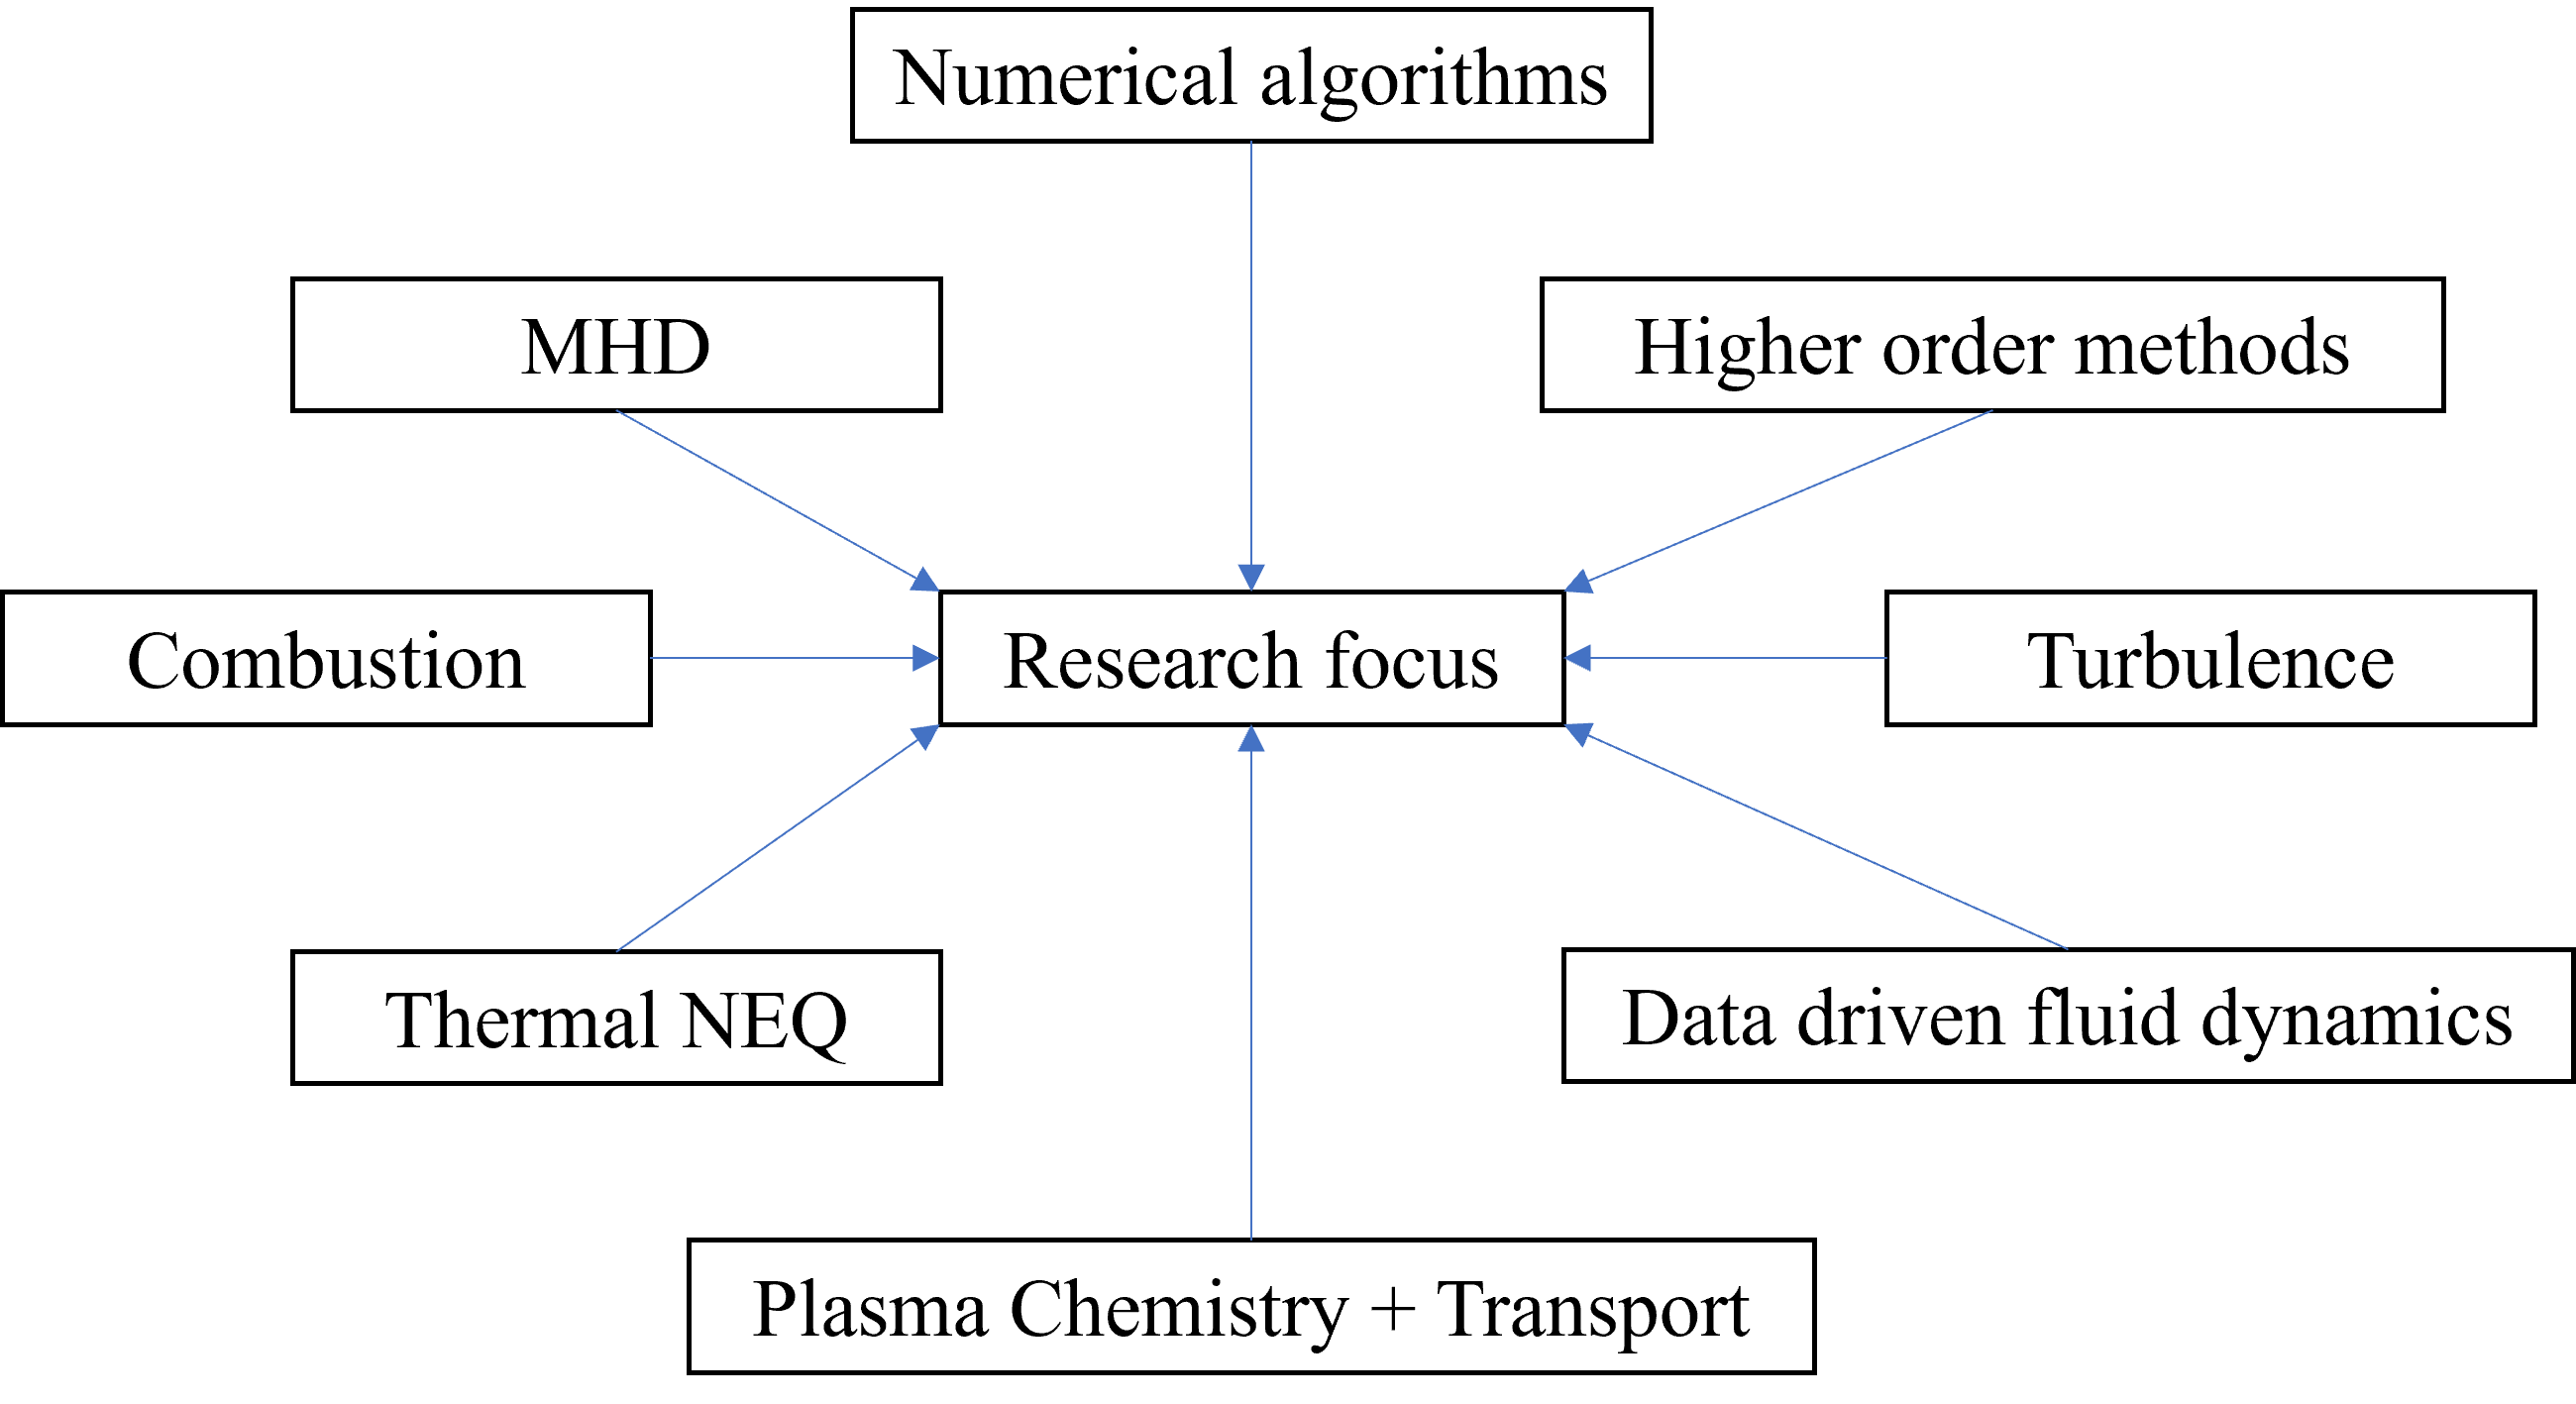
\includegraphics[width=0.5\textwidth]{figures/research_focus3.png}
  \end{center}
  \caption{Current and future research interests.}\vspace{-10pt}
  \label{fig:focus}
\end{wrapfigure}\vspace{0pt}
\noindent In my career as an \textbf{Assistant Professor} at the IIT Madras, I will \textbf{study the fundamental physics to solve the problems that limit high speed vehicle design}, such as thermal protection, communication blackouts, and turbulence. This will be a general advance in the field that will be achieved by \textbf{developing novel} computational fluid dynamic (\textbf{CFD}) models for \textbf{hypersonic flow physics}.   
\noindent Ground and flight tests are an integral part of spacecraft development, and computers, through CFD, bridge the gap between them. Throughout my research journey, I have created CFD codes that use numerical algorithms for unstructured grids with high-performance computing to explore different aspects of hypersonic flight, such as plasma, aerodynamics, flow control, and propulsion. My current and future research interests can be visualized in Fig. \ref{fig:focus} as a combination of different fundamental areas \textbf{relevant to developing hypersonic vehicles}.
\vspace{-10pt}
\begin{figure}[H]
    %\centering
     \begin{minipage}{.45\textwidth}
        \centering
        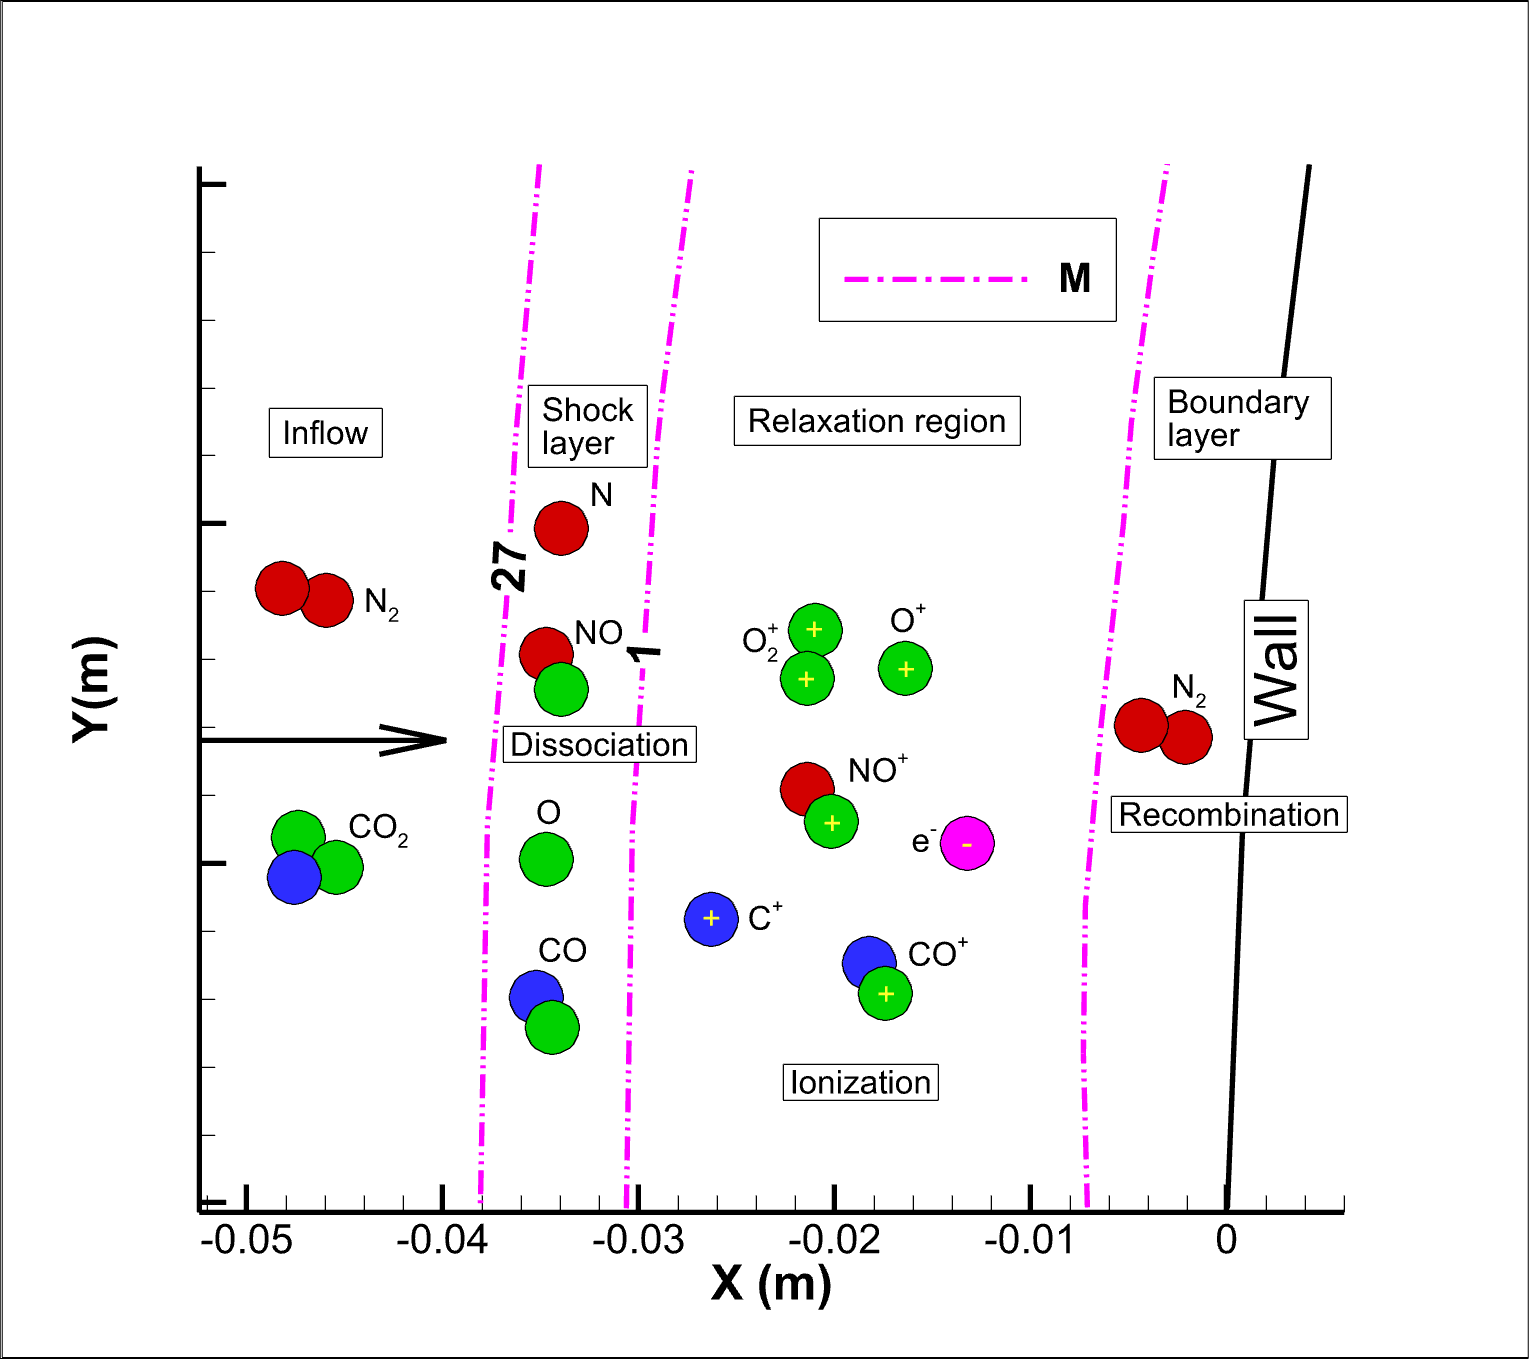
\includegraphics[trim={2cm 1cm 1cm 3cm},clip,scale=0.17]{figures/flowfeatures_molecules_noT_CO2_2.png}
        \caption{Flow ionization in Martian atmosphere [M=Mach no.]\cite{sharma2024mhd}.}%\vspace{-10pt}
        \label{fig:exomars_ionization}
    \end{minipage}
    \hfill
    \begin{minipage}{0.45\textwidth}
        \centering
        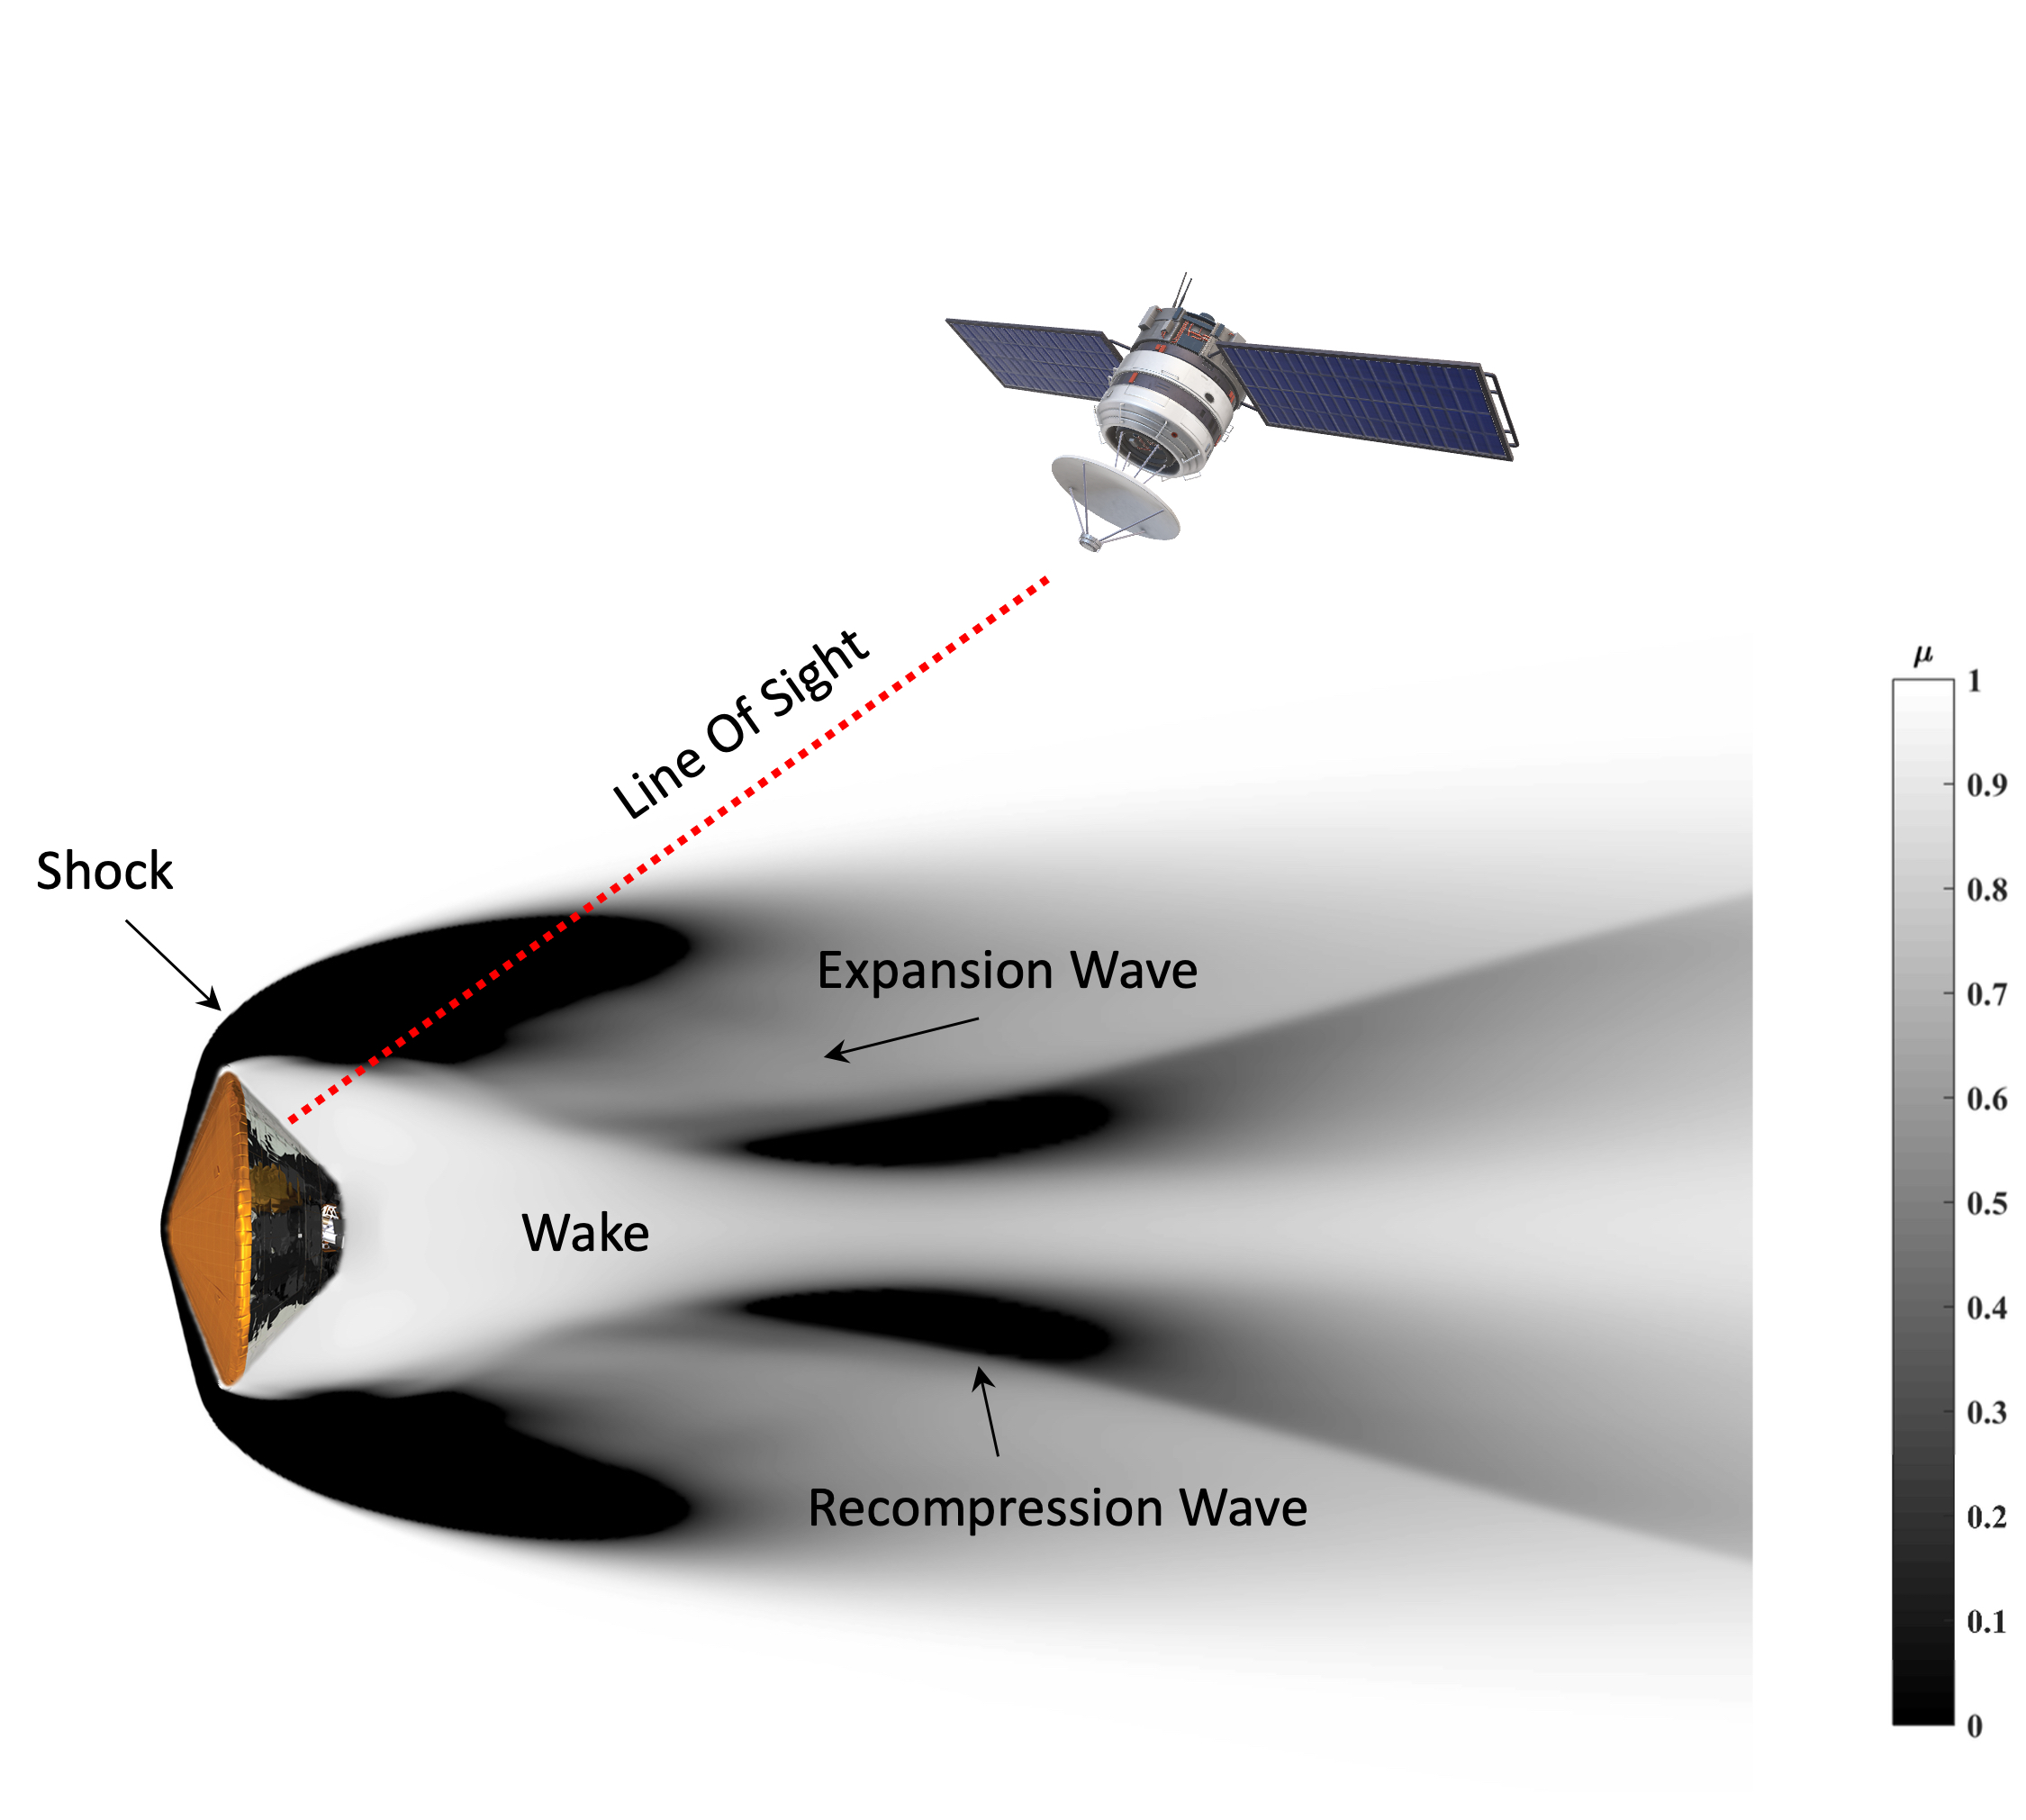
\includegraphics[trim={1.5cm 5cm 18cm 12cm},clip,scale=0.13]{figures/Flow_Sketch.jpg}
        \caption{Plasma around re-entry capsule\cite{giangaspero20233d}.}%\vspace{-10pt}
        \label{fig:blackout}
    \end{minipage}
\end{figure}\vspace{-15pt}
\noindent When a \textbf{spacecraft} enters into a planet's atmosphere, it travels at \textbf{hypersonic speeds} creating a strong bow shock wave that significantly increases the temperature and pressure, leading to \textbf{thermal and chemical non-equilibrium (TCNEQ)} in the flow, as seen in Fig. \ref{fig:exomars_ionization}. This plasma formation leads to two challenges: \textbf{excessive spacecraft surface heating and radio communication blackout}, as illustrated in Fig. \ref{fig:blackout}, where the shading intensity represents blackout severity\cite{sharma2024mhd,giangaspero20233d}. \\
%\textbf{My future research projects are rooted in the idea of developing new solutions to mitigate these challenges by studying their underlying physics}.\\
Developing \textbf{reusable thermal protection systems} adaptable to various planetary atmospheres necessitates investigating \textbf{new technologies} such as magnetohydrodynamics; \textbf{MHD}. For example, on a round trip to Mars, a spacecraft has to enter the Martian and the terrestrial atmosphere, which are distinctively different. As the plasma is inherently electrically conductive, this approach can open new directions for heat management and blackout mitigation during atmospheric entry. This multi-physio-chemical flow is solved by \textbf{coupling the Maxwell equations with TCNEQ Navier Stokes} equations. To explore the physics of atmospheric entry in the presence of MHD, I have \textbf{developed COMET} during my postdoc at KU Leuven, Belgium, which is an \textbf{implicit, 3D finite volume (FV) unstructured grid CFD code} in the COOLFluiD platform, written in C++\cite{sharma2024mhd}. I wrote a Python library integrated within COMET to simulate the magnetic field generated by a finite-sized magnet of different shapes and orientations. Using COMET, I investigate the plasma-MHD interactions \textbf{to develop methods for using magnets in the heat shield assembly, as seen in Fig. \ref{fig:exomars_magnet}\cite{sharma2024mhd}, that divert the Martian and terrestrial (or indeed any arbitrary planet's) atmospheric plasma to minimize heat shield ablation}.
\par
\begin{wrapfigure}{r}{0.3\textwidth}
  \begin{center}
  \vspace{-15pt}
    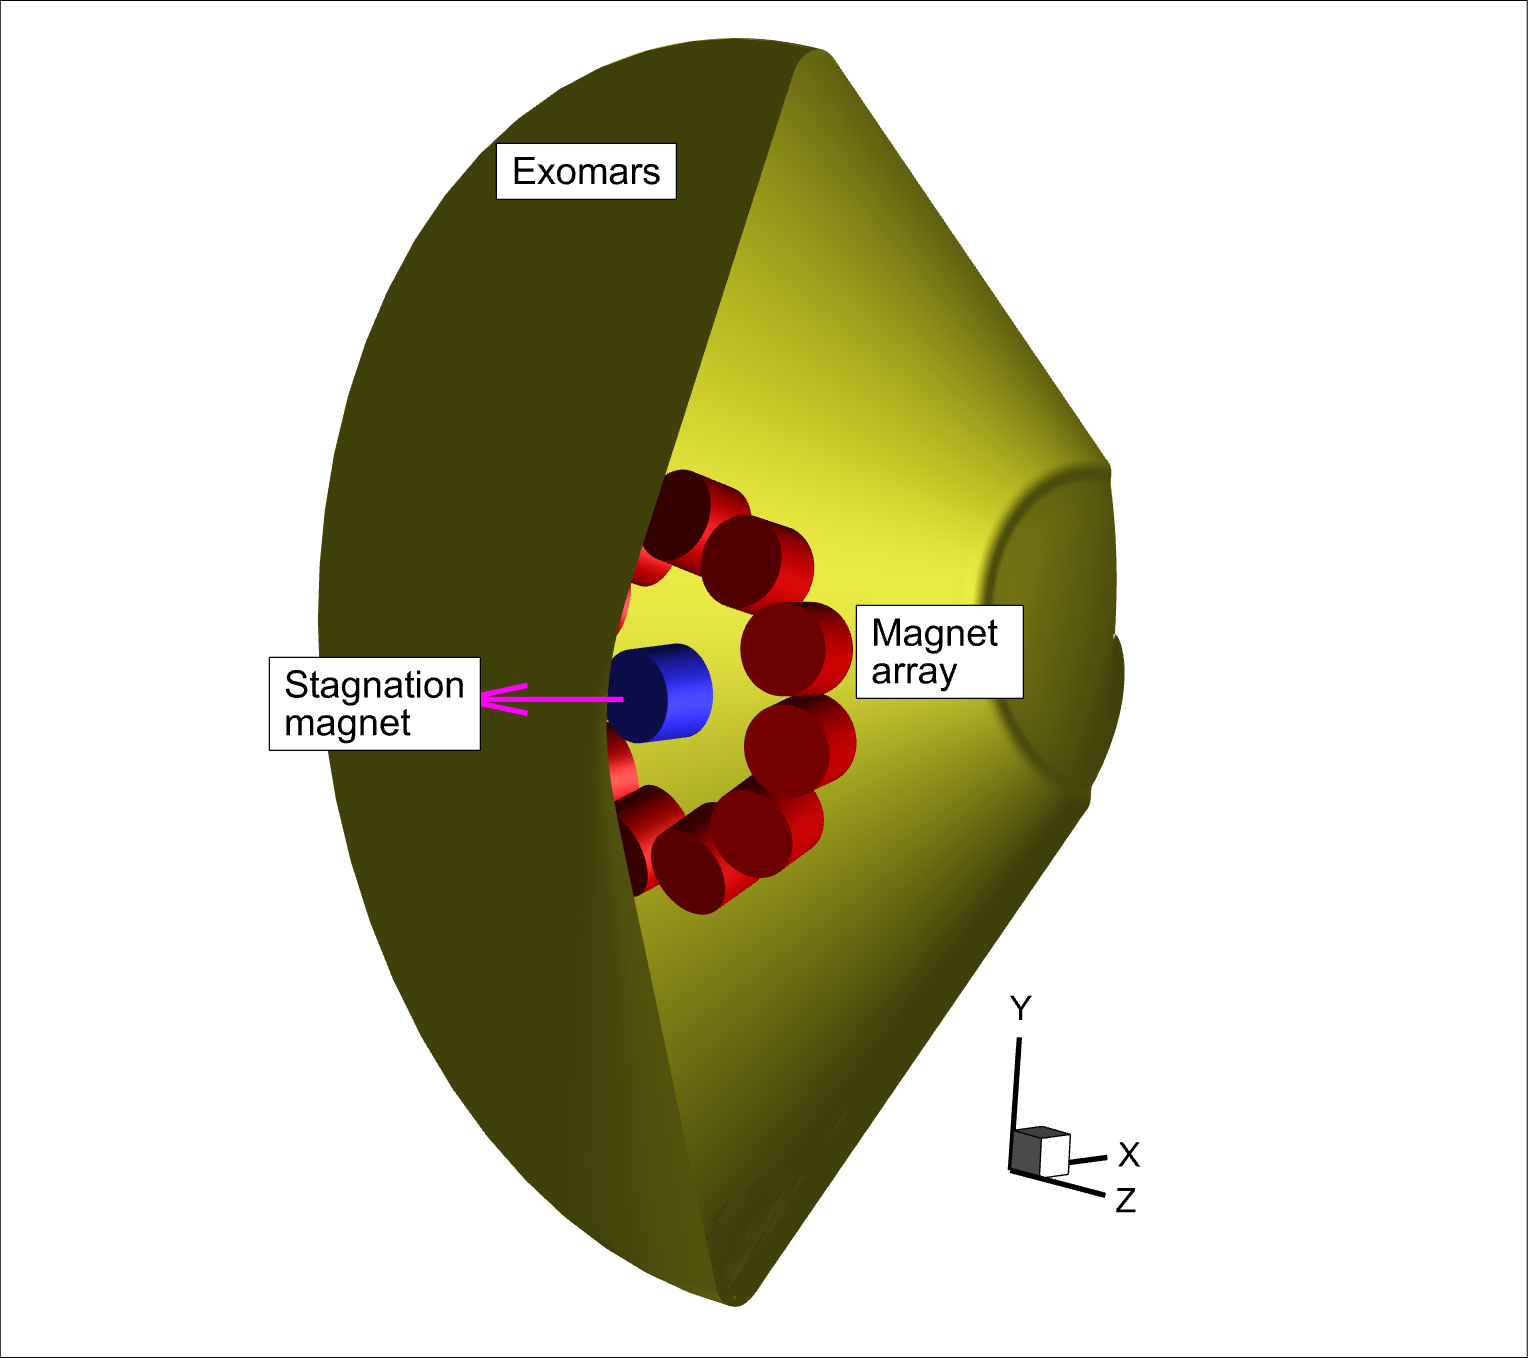
\includegraphics[trim={9cm 1cm 13cm 1cm},clip,scale=0.13]{figures/3D_exomars_caseC.png}
  \end{center}
 \caption{MHD heat shield \cite{sharma2024mhd}.} \label{fig:exomars_magnet} \vspace{-12pt}
%\end{wrapfigure}
%\begin{wrapfigure}{r}{0.3\textwidth}
  \begin{center}
  %\vspace{-30pt}
     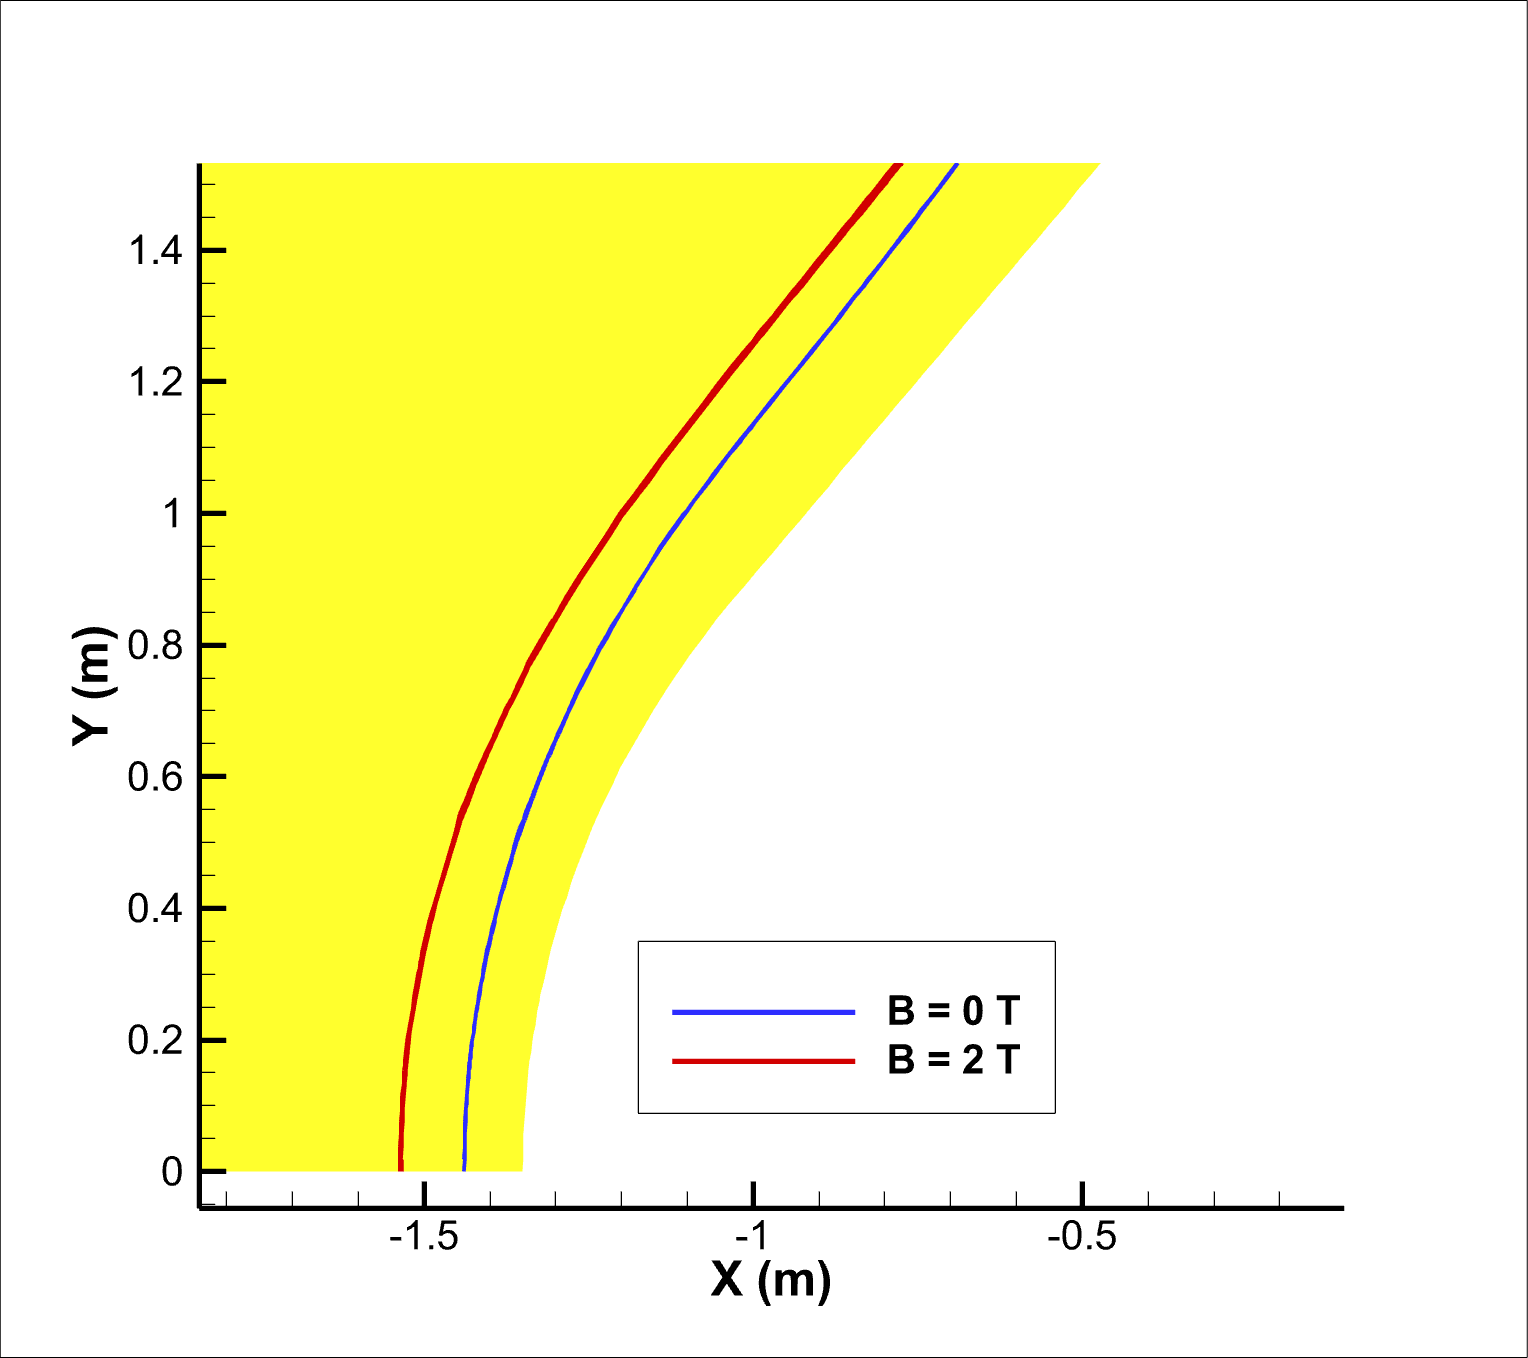
\includegraphics[trim={2cm 5cm 16cm 5cm},clip,scale=0.12]{figures/ssd_full_magnet_new.png} 
 \caption{Change in SSD for different magnetic field strength \cite{sharma2024mhd}.}
 \label{fig:exomars_ssd}%new fig needed
 \end{center}
 \vspace{-20pt}
\end{wrapfigure}
\noindent Fig. \ref{fig:exomars_ssd}\cite{sharma2024mhd} shows the change in shock standoff distance (SSD) due to the magnetic field at peak heating conditions during the Martian entry of the ExoMars capsule. The increase in SSD due to MHD results in a decrease in heatflux on the forebody of the capsule, thus demonstrating the scope of this method.
 % why this library is important, explain in 1-2 lines.
\noindent The \textbf{plasma sheath} absorbs, reflects, or scatters radio signals, effectively disrupting communications between the spacecraft and ground control, thus creating a \textbf{radio communication blackout}, as shown in Fig. \ref{fig:blackout}, that can last for several minutes. This phenomenon is a significant concern for mission safety and operational control. Characterizing and predicting this communication blackout phase is an important step toward mitigating it. Therefore, I co-developed a blackout prediction code in Python with a PhD student in my group\cite{giangaspero20233d}, where we \textbf{couple the fields of geometric optics with electromagnetics} through Eikonal equations. The solver takes the non-magnetized atmospheric entry results from COMET as input and calculates plasma optical properties relevant to communication blackout. 
\noindent We then calculate the vehicle's radar cross section (RCS) using far-field theory, thus visualizing the communication window during a planetary atmospheric entry\cite{giangaspero2024raytracing}. 
Using the code, we can predict the signal path and its attenuation caused by reflections and refractions with plasma. 
%\noindent \textbf{\textcolor{red}{For my first research project at UAT}}, I will develop models for calculating the transport properties of magnetized plasma. 
However, the Lorentz force generated by the magnetic field on electrons results in their helical motion around local magnetic field lines. This leads to the Hall effect, which arises from the differential motion of electrons and ions across magnetic fields, and the ion-slip effect, which accounts for the relative drift between ions and neutral particles\cite{bruno2008transport}. The models used to calculate plasma transport properties, such as electrical conductivity, viscosity, and thermal conductivity in COMET and blackout code, use the collision frequency of plasma constituents. At very low pressures that exist at higher altitudes on Earth and other planets, such as Mars, the helical motion frequency, also known as the cyclotron frequency, is higher than the collision frequency of plasma, breaking the isotropy of the system. Therefore, there is a need to \textbf{develop theoretical and computational models} that account for cyclotron frequency, Hall, and ion-slip effects in calculating transport matrices obtained by solving the Boltzmann Equation through Chapman-Enskog expansion. 
\vspace{-5pt}
\begin{figure}[H]
   \centering
%\begin{minipage}{0.65\textwidth}
%        \centering
         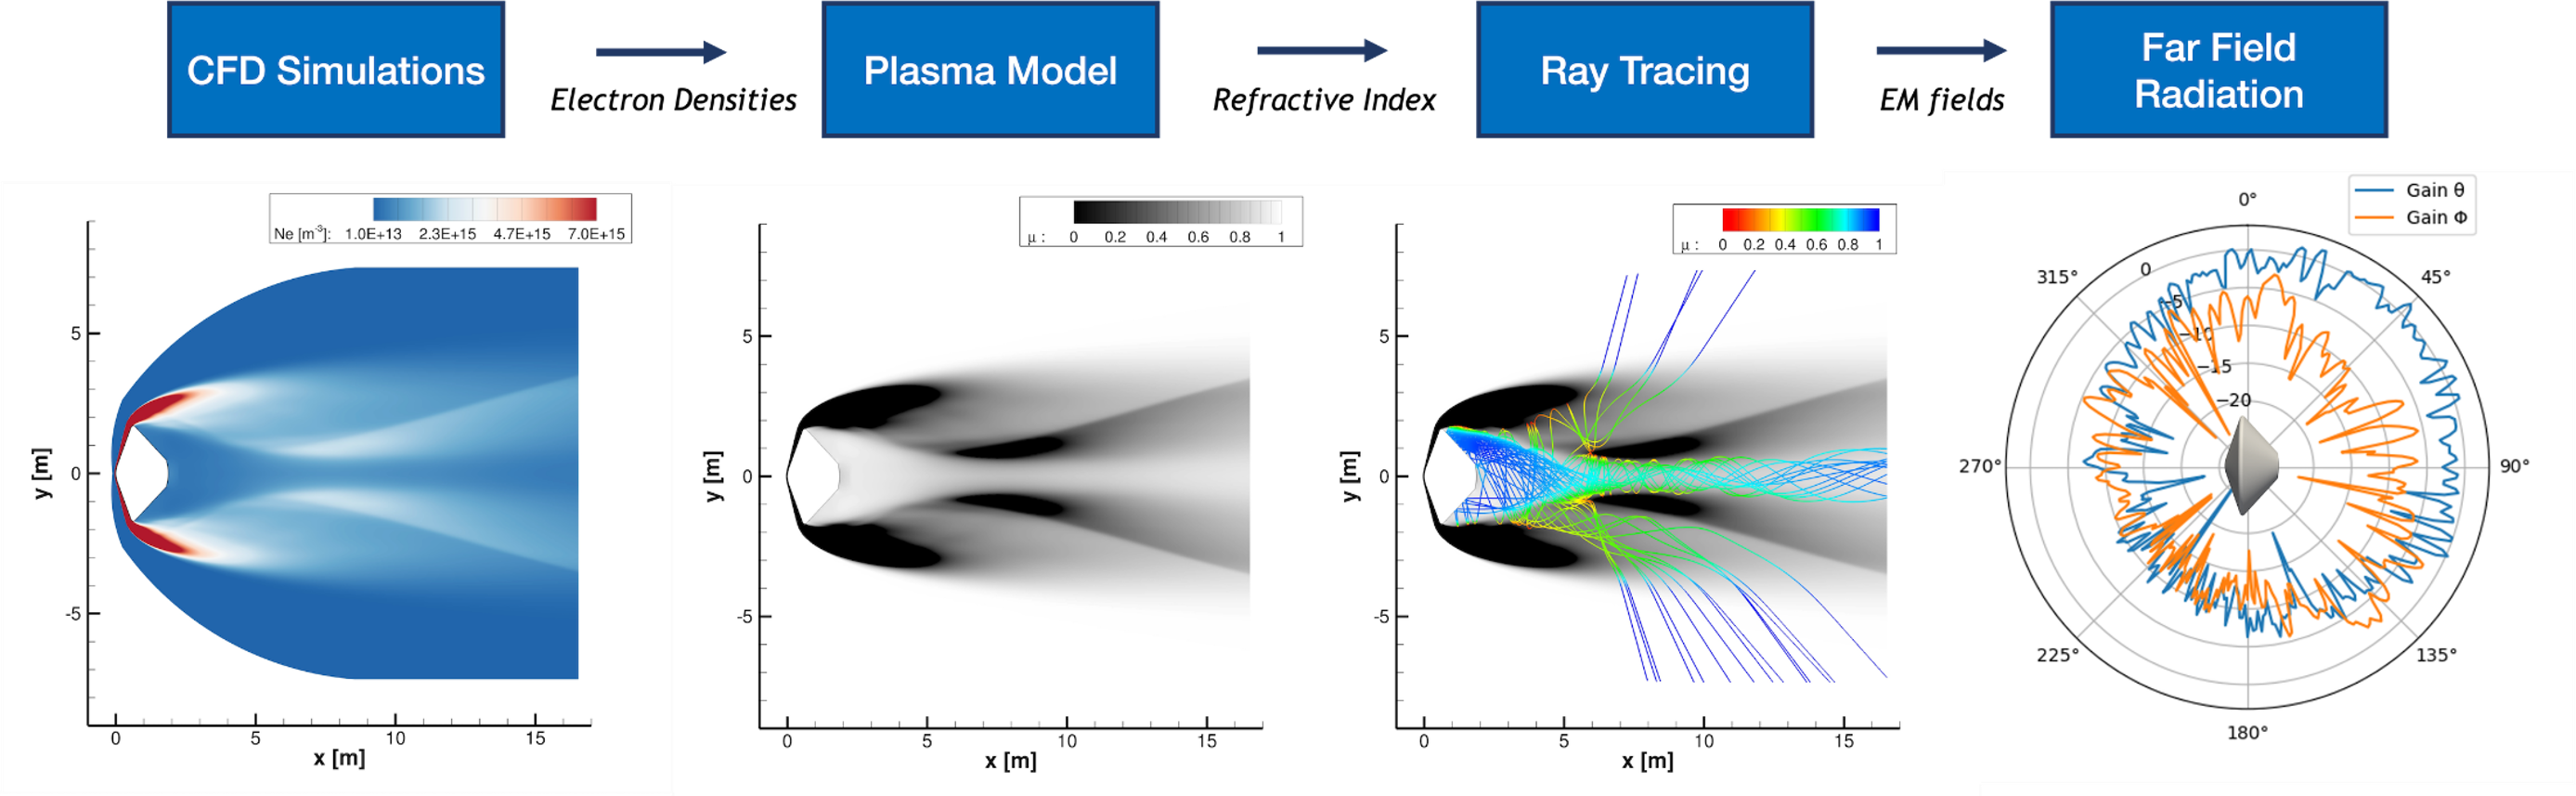
\includegraphics[trim={1cm .1cm 0.11cm 0.1cm},clip,scale=0.5]{figures/algo.png}
        \caption{Steps involved in characterizing radio blackout.\cite{sharma2024mhd, giangaspero20233d, giangaspero2024raytracing}}\vspace{-15pt}
        \label{fig:blackout_algo}
%    \end{minipage}
\end{figure}%\vspace{-10pt}
%Together with COMET, for given ambient conditions and entry speed, we can numerically characterize blackout for a given antenna frequency. This creates a unique state-of-art package, as seen in Fig. \ref{fig:blackout_algo}. 
\noindent The absorption, reflection, and scattering \textbf{characteristics of electromagnetic (EM) waves are modified in the presence of the anisotropic magnetized plasma}, thus potentially reducing signal attenuation and mitigating communication blackout. To reliably analyze radio blackout, a CFD solver like COMET that models the effect of MHD on plasma during atmospheric entry is required. Due to the lack of such codes in the literature, there has been very little progress in studying blackout mitigation along with heat flux management using MHD.\\ 
Therefore, \textbf{\textcolor{red}{as my first project}, I will develop a state-of-the-art package, shown in Fig. \ref{fig:blackout_algo}, that will contribute towards developing reusable thermal protection systems while sending data without interruption during atmospheric entry} on different planets while increasing our understanding of the interaction of EM waves with magnetized plasma. This project will also develop anisotropic transport property models for magnetized plasma, which will increase the fidelity of the solution, which is essential to developing new MHD-based technologies. 
These new computational models for communication signal characterization and RCS calculation, coupled with CFD to account for magnetized plasma properties, will be a novel contribution to the field. 
%\textbf{\textcolor{red}{Therefore, in my first research project at UAT}}, I will develop a complete state-of-the-art package computational models that analyze the effect of MHD on the mitigation of radio communication blackout during atmospheric entry. 
%This project will develop a new thermo-physics library in C++ that will be integrated with COMET to study the effect of anisotropic magnetic transport properties during MHD entry in a planetary atmosphere, which is essential to developing new MHD-based technologies. \textbf{\textcolor{red}{Therefore, in my first research project at UAT}}, I will develop a complete state-of-the-art package computational models that analyze the effect of MHD on the mitigation of radio communication blackout during atmospheric entry. 
%I can reduce the below. Not very innovative, but can be funded.
\par
\begin{wrapfigure}{l}{0.41\textwidth}
  %\begin{center}
  \vspace{-15pt}
    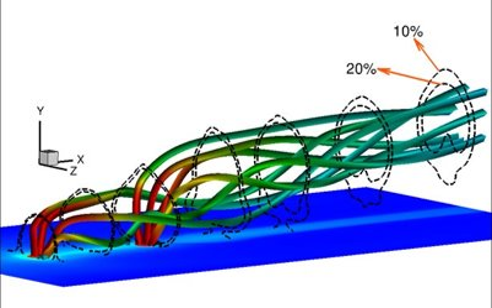
\includegraphics[trim={0.2cm 0.5cm 0.5cm 0.5cm},clip,scale=0.55]{figures/crv_scramjet.png}
  %\end{center}
  \caption{Counter rotating vortex formed due to shock-induced air-fuel mixing (shown by contours) inside SCRAMJET combustor\cite{sharma2020effect}.} %\vspace{-11.5pt}
  \label{fig:scramjet2}
%\end{wrapfigure}
%\begin{wrapfigure}{r}{0.3\textwidth}
  %\begin{center}
  %\vspace{-30pt}
     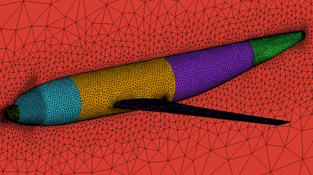
\includegraphics[trim={0cm 0cm 0cm 0cm},clip,scale=0.8]{figures/Unstructmesh.png}
 \caption{High aspect unstructured grid mesh for simulating DLR F6 with Jatayu\cite{sharma2022development}.}\vspace{-11pt}
\label{fig:unstrutcmesh}
 %\end{center}
 \vspace{-2pt}
\end{wrapfigure}
%\begin{wrapfigure}{l}{0.4\textwidth}
%  \vspace{-10pt}
%    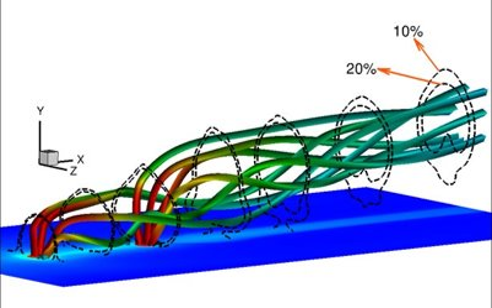
\includegraphics[trim={0.2cm 0.5cm 0.5cm 0.5cm},clip,scale=0.55]{figures/crv_scramjet.png}
%  \caption{Counter rotating vortex formed due to shock-induced air-fuel mixing (shown by contours) inside SCRAMJET combustor.} \vspace{-11.5pt}
%  \label{fig:scramjet2}
%\end{wrapfigure}
%\vspace{-11.5pt}
\noindent  \textbf{Hypersonic cruise vehicles} (HCV) utilize air-breathing engines like supersonic RAMJET (\textbf{SCRAMJET}) engines for propulsion. During my Ph.D., I explored the shock-induced turbulent \textbf{air-fuel mixing interaction physics} at high speeds inside SCRAMJET engines, as seen in Fig. \ref{fig:scramjet2}, to provide a set of design rules\cite{sharma2020computational, sharma2020determination,sharma2020effect, sharma2020effect2, sharma2022influence}.
\noindent To fulfill this objective, I \textbf{developed Jatayu, a 3D FV unstructured grid, general-purpose CFD code for turbulent high-speed flows in C++}. It models turbulence using different Reynolds-Averaged Navier-Stokes (RANS) models\cite{sharma2022development}. Although \textbf{FV is robust} and can handle high aspect ratio meshes used in practical aerospace applications, as shown in Fig. \ref{fig:unstrutcmesh}, \textbf{the stencil increases with increasing order of accuracy}, which leads to complexities near the boundary as seen in Figs. \ref{fig:stencil_2O} and \ref{fig:stencil_3O}, where the solid thick black line represents the boundary of the computational domain and the corresponding ghost cells, the green cells are immediate neighbors, and pink are neighbor of neighbor for the quadrilateral cell used for calculation, shown in yellow. \textbf{Larger stencils are computationally expensive} while requiring complex extrapolation functions for high aspect unstructured grids. \textbf{High-order numerical methods such as the flux reconstruction (FR)\cite{huynh2007flux} offers a promising alternative}, providing greater accuracy per degree of freedom while reducing numerical errors without significant computational cost increases. 
%\par
%\begin{wrapfigure}{l}{0.4\textwidth}
%  \vspace{-10pt}
%     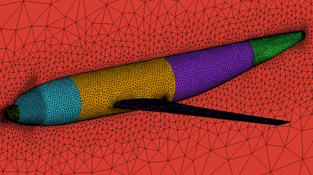
\includegraphics[trim={0cm 0cm 0cm 0cm},clip,scale=0.8]{figures/Unstructmesh.png}
%        \caption{High aspect unstructured grid mesh for simulating DLR F6 with Jatayu.}\vspace{-11pt}
% \label{fig:unstrutcmesh}
%\end{wrapfigure} %\vspace{-3pt}
FR unifies various Finite Element (FE) and FV schemes by reconstructing a globally continuous flux from local discontinuous solutions using correction functions. FR \textbf{retains the stencil of 2nd order FV} shown in Fig. \ref{fig:stencil_2O} while using Lagrange polynomials distributed along solution points within a single cell \textbf{to deliver higher order solution accuracy}. Therefore, high-order accuracy can be achieved even on a lower-quality mesh because of the degrees of freedom (DoF) introduced in each cell while giving better solution fidelity, as shown in Fig. \ref{fig:grid}. With my PhD student, I have \textbf{co-developed an open-source library for storing this high-order data} in an open-source CGNS (CFD General Notification System) data retrieval format\cite{dhib2024input}.
\begin{figure}[H]
    %\centering
     \begin{minipage}{.45\textwidth}
        \centering
        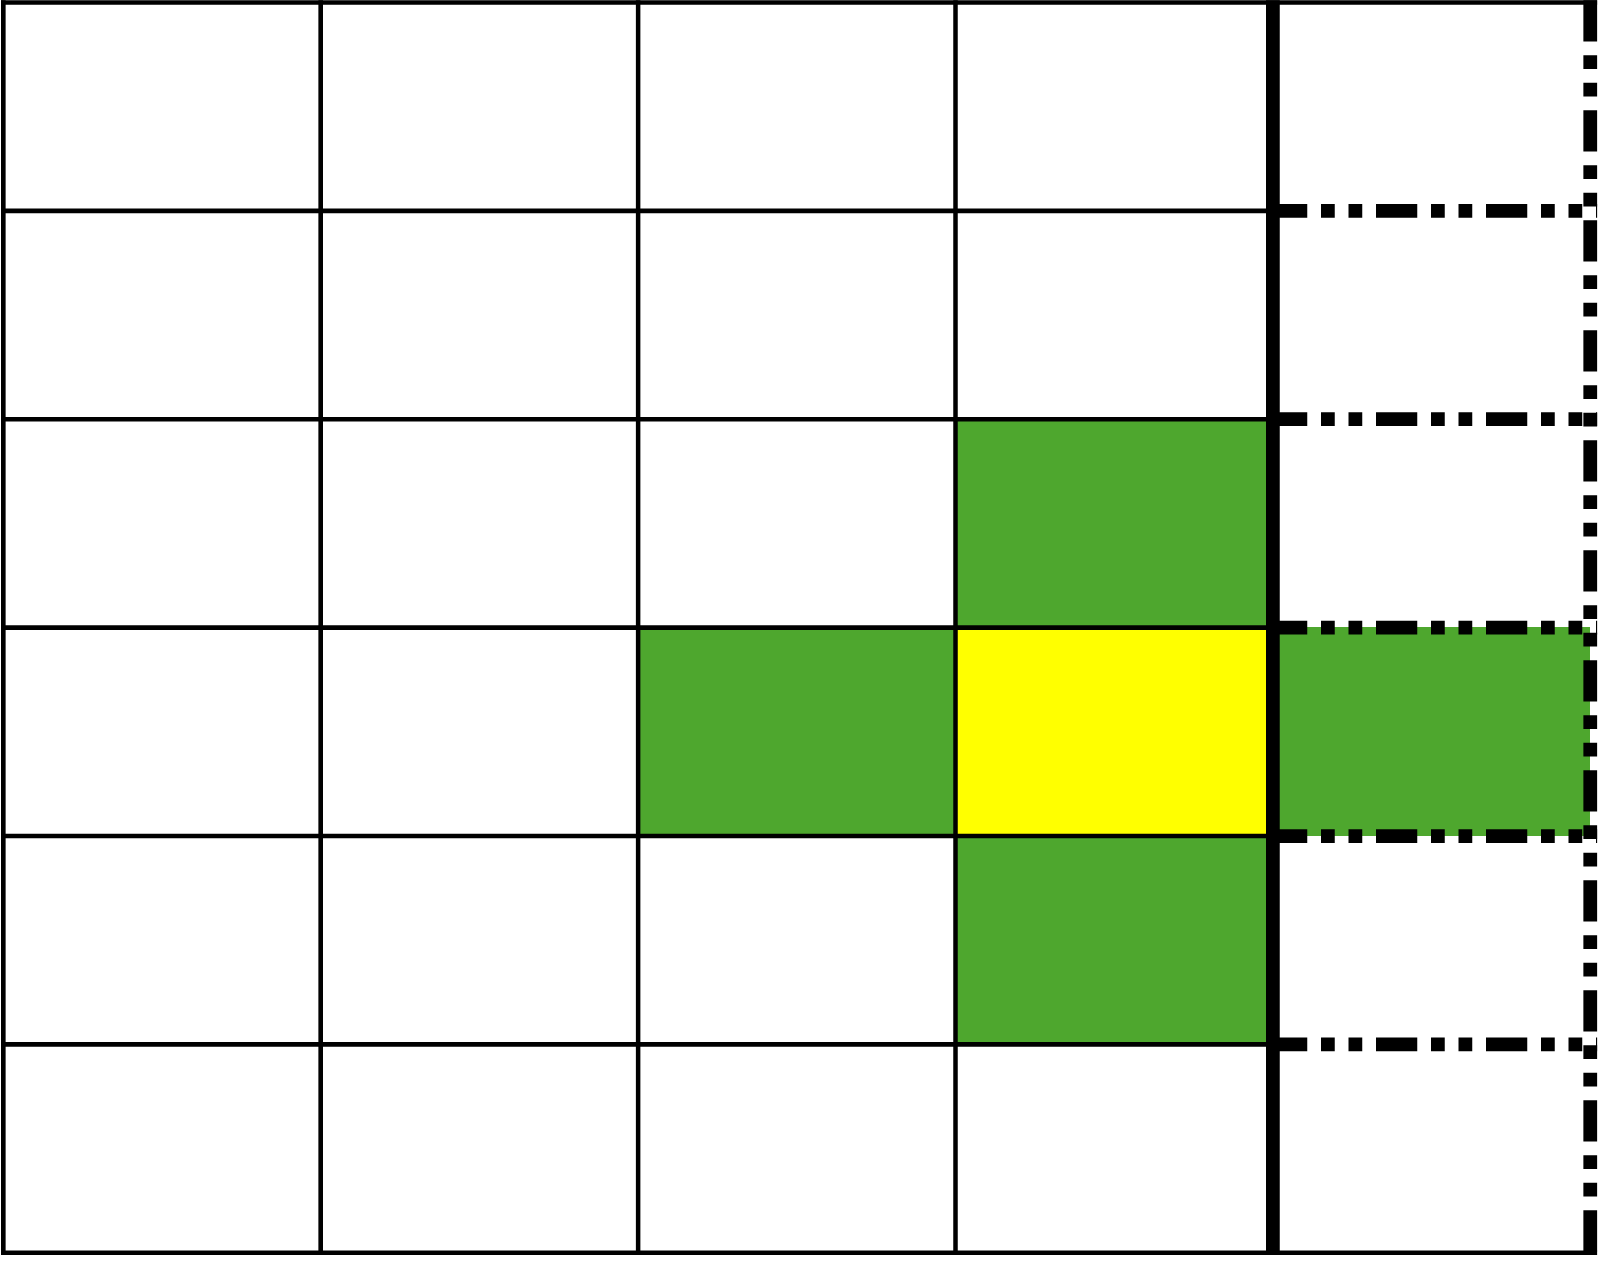
\includegraphics[trim={0cm 0cm 0cm 0cm},clip,scale=0.5]{figures/2nd_order_fv_BC.png}
        \caption{Stencil for 2nd order FV.}%\vspace{-10pt}
        \label{fig:stencil_2O}
    \end{minipage}
    \hfill
    \begin{minipage}{0.45\textwidth}
        \centering
        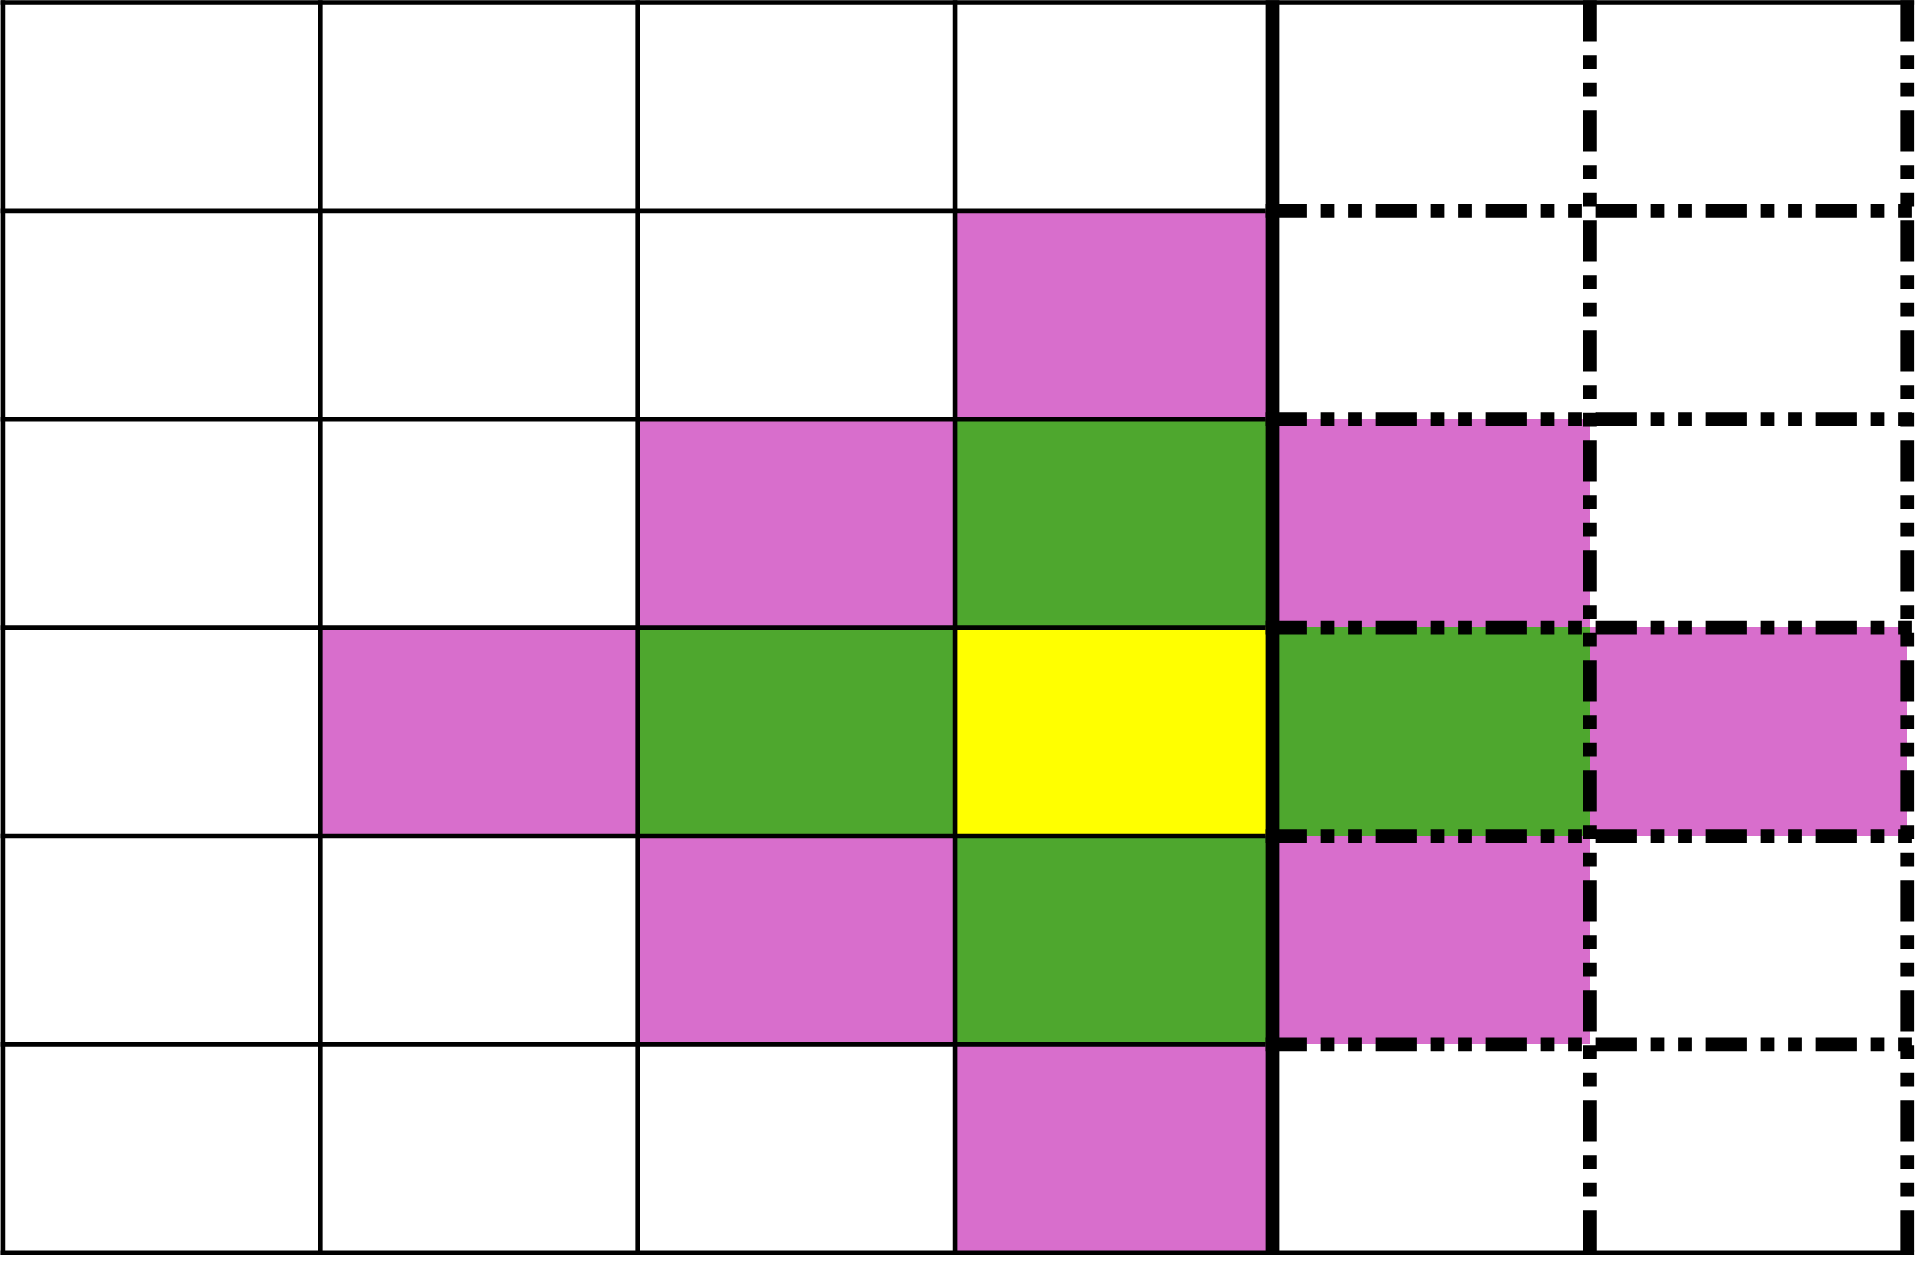
\includegraphics[trim={0cm 0cm 0cm 0cm},clip,scale=0.5]{figures/3rd_order_fv_BC.png}
        \caption{Stencil for 3rd order FV.}%\vspace{-10pt}
        \label{fig:stencil_3O}
    \end{minipage}
\end{figure} %droplet breakup study with FR. 
\noindent  When a \textbf{high-speed vehicle} such as rockets, super/hypersonic aircraft or missiles, and reentry vehicles, \textbf{interact with raindrops, it may result in surface cavitation}. At hypersonic speeds, impact with a single rain droplet can provide loads of up to $40$ kN to an extremely small area\cite{briggs2023experiments, briggs2024investigation}. Therefore, \textbf{impacts of this magnitude can lead to major structural damage to the vehicle}. Smaller droplets are affected by drag differently and are readily diverted from the fluid path, thus reducing this final impulsive loading. 
\par
\begin{wrapfigure}{l}{0.65\textwidth}
  \vspace{-10pt}
     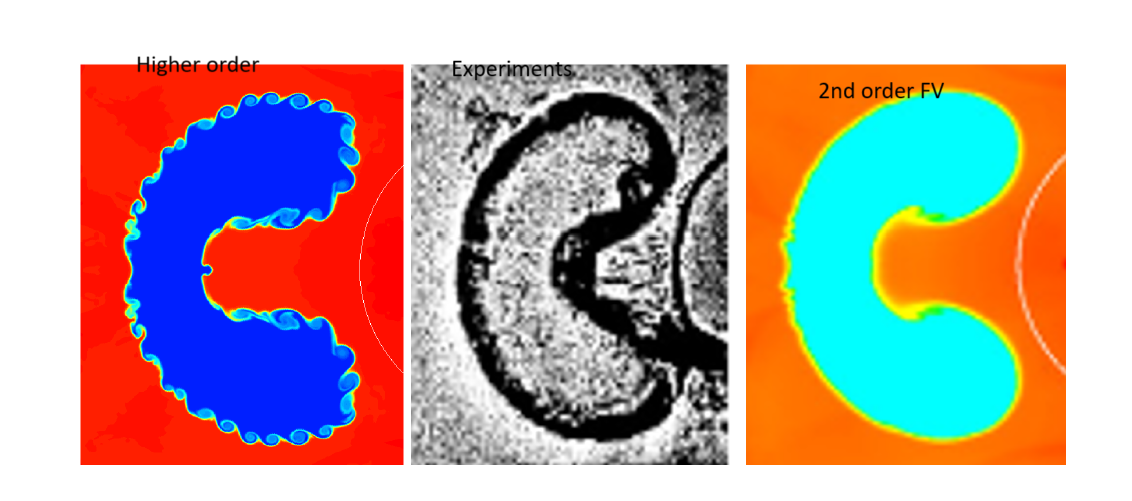
\includegraphics[trim={0.4cm 0.4cm 1cm 0cm},clip,scale=0.6]{figures/Heliumbubble.png} 
  \caption{Higher order vs Experiments vs $2^{nd}$ order FV\cite{peyvan2022oscillation}.}  \vspace{-11pt}
 \label{fig:drop_flux}
\end{wrapfigure}
\noindent Therefore, to \textbf{understand the structure loading, the droplet breakup character as it processes through the bow shock preceding the high-speed vehicle is quite important}. While droplet deformation is mainly guided by the Weber number, other factors can impact the propagation of the pressure wave through the droplet and ultimately change the breakup mechanism\cite{kondo2019simulation}. Due to the high temperature environment, the conventional thinking is that such droplets will immediately boil on impact with the shock due to the accompanying temperature rise. These boiling processes occur at a finite time that are limited by both convective heat transfer and latent heat physics which occur over much longer time scales than those associated with the droplet impact\cite{esplin2021measurement}. \textbf{I shall utilize the high fidelity FR framework to develop an understanding of the fluid (water, fuel) droplet breakup mechanism upon interaction with shockwave} along with boiling and shear-based breakup mechanism as \textcolor{red}{\textbf{my second project}}. To achieve this, the Volume of Fluid (VOF) method, that tracks different fluids in a single computational domain, must be integrated with the compressible flow FR solver, thus resulting in a high order multi-fluid, multi-scale, unstructured grid, CFD solver development. \textbf{FR is integral to resolving this multi physics phenomena}, as it has been seen in the literature\cite{peyvan2022oscillation} that the high fidelity offered by the higher order methods help in resolving the instabilities generated during interaction between Helium gas bubble with a moving shock, as observed in the experiments, are smeared by 2nd order FV unlike the higher order method, \textbf{as seen in Fig. \ref{fig:drop_flux}}.  %multi fluid solver in VHO framework needs to be developed. add references, and we are done.%Since we can \textbf{deploy relatively coarser meshes for very high order (VHO) FR, as seen in Fig.\ref{fig:grid}, complex mesh generation steps can be avoided} in practical aerospace applications. 
%This is essential to efficiently performing complete 3D simulations of TCNEQ flows involving atmospheric entry vehicles. Several flow features, such as the effect of turbulence, evaluation of cross-flow vortices over the vehicle body, evaluation of instabilities, and the effect of the angle of attack, cannot be simulated in 2D axi-symmetric simulations. Therefore, these \textbf{3D high-fidelity simulations are important in exploring complex physics encountered during hypersonic flights and thus will reduce vehicle development times}.
%However, \textbf{applying FR to TCNEQ flows is quite tricky}, as in higher-order frameworks, \textbf{improper handling of multi-species, high-temperature flows leads to numerical instabilities and non-physical solutions}, such as negative densities or pressures. To overcome these challenges, I will \textbf{develop entropy-stable, positivity-preserving schemes relevant to multi-species flows} as my \textbf{\textcolor{red}{second research project}} that can be applied to non-equilibrium flows. This development will be a general advance in the field since such numerical schemes have not been developed in FR for non-equilibrium flows. 
\begin{comment}
\begin{figure}[H]
    %\centering
     \begin{minipage}{.4\textwidth}
        \centering
        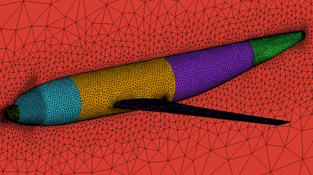
\includegraphics[trim={0cm 0cm 0cm 0cm},clip,scale=0.8]{figures/Unstructmesh.png}
        \caption{High aspect unstructured grid mesh for simulating DLR F6 with Jatayu.}%\vspace{-10pt}
        \label{fig:unstrutcmesh}
    \end{minipage}
    \hfill
    \begin{minipage}{0.6\textwidth}
        \centering
        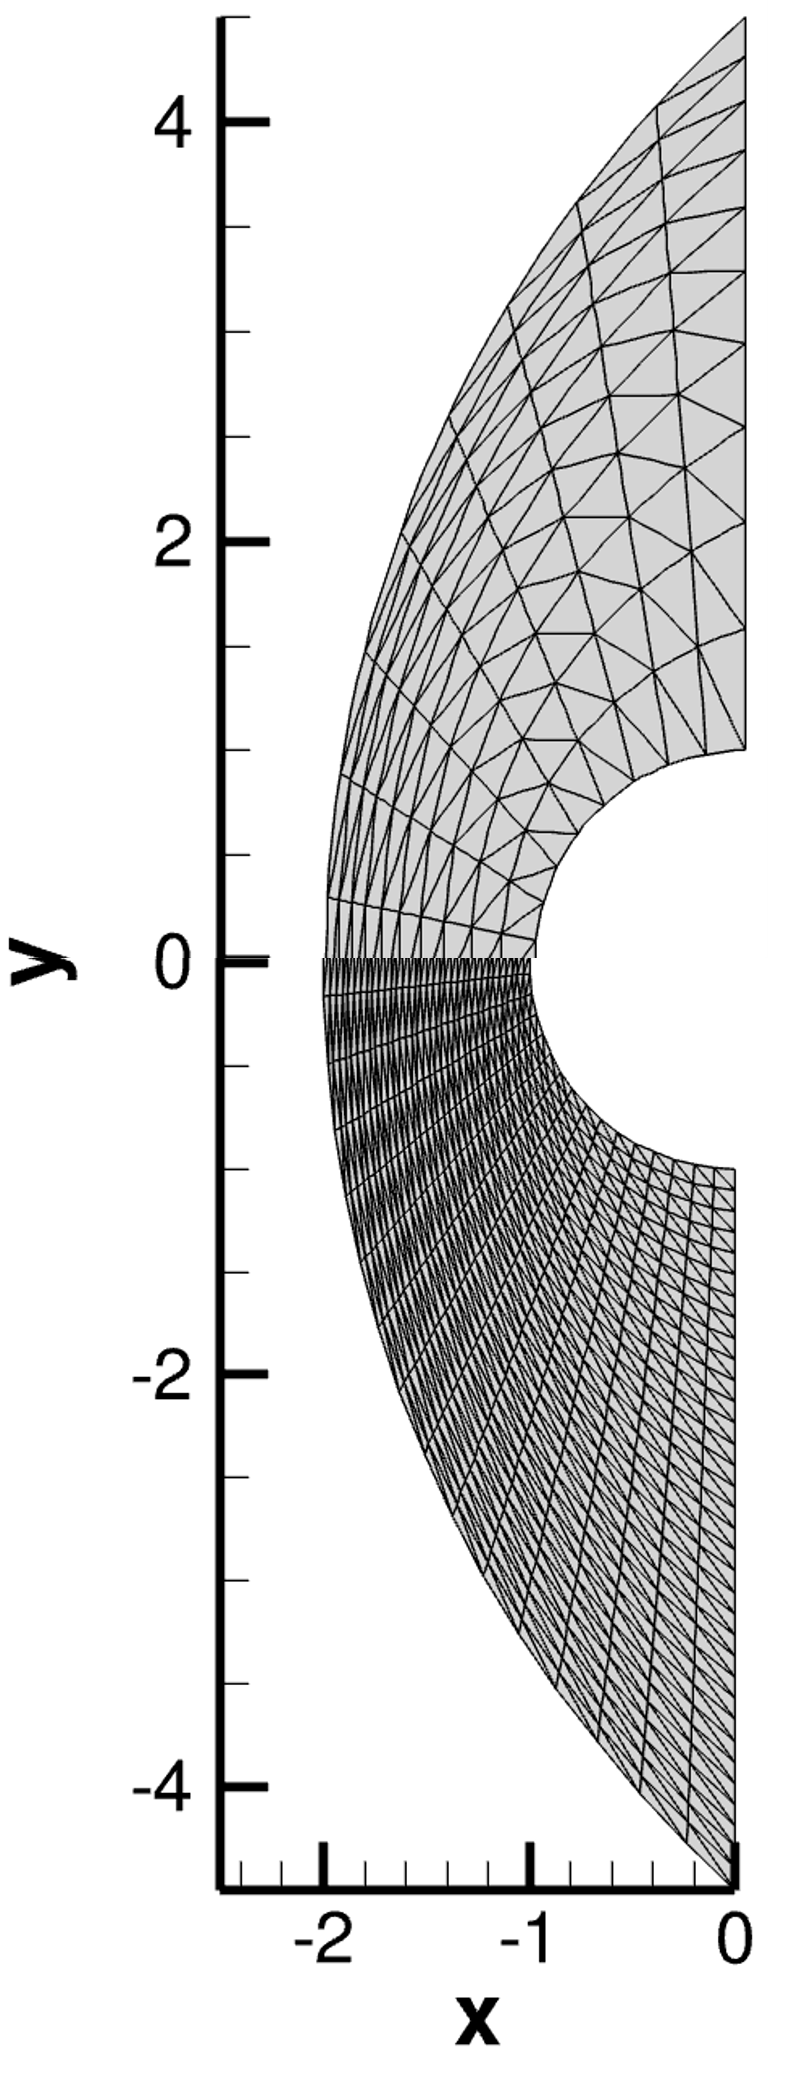
\includegraphics[trim={1cm 0.8cm 1cm 0cm},clip,scale=0.6, angle = -90]{figures/HO_vs_FVM.png}
        \caption{FV (left) vs FR grid (right).}%\vspace{-10pt}
        \label{fig:grid}
    \end{minipage}
\end{figure}
\end{comment}
\par
\begin{wrapfigure}{r}{0.15\textwidth}
  \vspace{-10pt}
     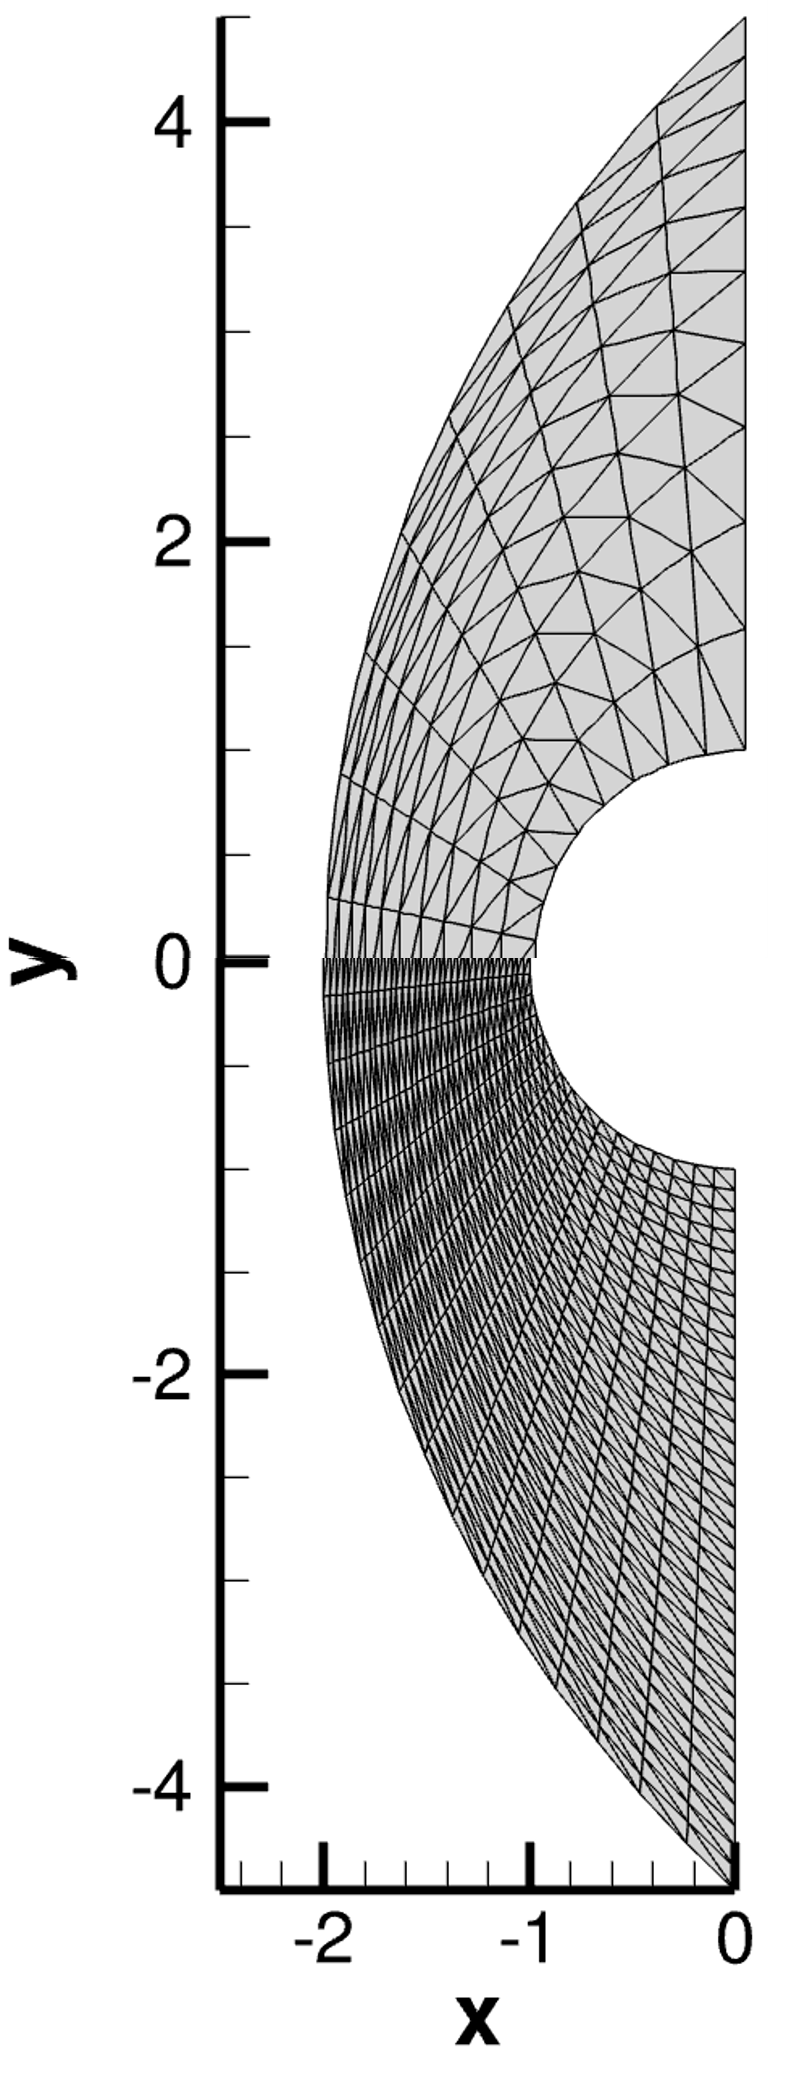
\includegraphics[trim={1cm 0.8cm 1cm 0cm},clip,scale=0.6]{figures/HO_vs_FVM.png} 
  \caption{FR (top) vs FV grid (bottom).}  \vspace{-11pt}
 \label{fig:grid}
\end{wrapfigure} \vspace{-3pt} %rewite the below on LES with FR for LTT and develop RANS data driven models for hypersonic flow and for LTT. 
\noindent \textbf{Turbulent boundary layers generate $5$–$10$ times greater heat flux} and skin friction than their laminar counterparts. Therefore, it is \textbf{advantageous to maintain a laminar boundary} layer over the surface of aerospace vehicles. Moreover, hypersonic flight is characterized by the presence of strong shocks, which interact with the vehicle boundary layer and strongly influence the aerodynamic and heat loads. \textbf{The limitation in knowledge of when, where, and how boundary layer transition will happen, especially in the presence of shocks during flight, hinders the design and development} of next-generation hypersonic vehicles such as high-speed interceptors, reusable launch vehicles (RLV), and HCV\cite{berry2011recommendations}. \\
\noindent Even though the stability and \textbf{laminar to turbulence transition (LTT) of boundary layers at supersonic and hypersonic speeds} along with their interactions with shockwaves have been studied separately and together for more than 50 years, much of the \textbf{complex physics remains unresolved} due to the extreme operational conditions during hypersonic flight, which needs to be urgently addressed for development of next generation hypersonic vehicles\cite{knight2018hypersonic}.
Although there is an \textbf{abundance of Direct Numerical Simulation (DNS)\cite{huang2025laminar} and Large Eddy Simulation (LES)}\cite{fu2021shock} simulations to explore the LTT physics, these methods are extremely computationally expensive and, therefore, still \textbf{far from usability in practical design applications}, such as in Fig. \ref{fig:unstrutcmesh}. Hence, \textbf{RANS modeling of turbulent flow} is still the choice as a design tool in the aerospace sector due to its low computational cost and its ability to capture relevant flow physics on high aspect unstructured grids. Moreover, the \textbf{second mode instability along with all different transition mechanisms should be included} in the RANS model to result in accurate prediction of LTT. It has been reported in the literature that the RANS models over predict heatflux and wall shear stress, even after accounting for various corrections to the models, which is traced to modeling of Reynold stress tensor\cite{DURAISAMY20251}. Therefore, \textbf{data driven turbulence modeling by coupling a neural network} can be a solution to modeling LTT and Reynolds stress tensor by training the models on available experimental and numerical datasets using DNS and LES simulations\cite{danvin2019laminar, bhatnagar2019prediction, paredes2020toward, parish2024data}. Therefore, as \textbf{\textcolor{red}{my third project}, I will work on developing data driven RANS models for simulating shock dominated turbulent hypersonic flows on various geometries within the higher order framework}. The model will be trained for Reynolds stress tensor closure and identifying instabilities in hypersonic flows through neural networks, for application of accurate prediction of anisotropic turbulence and transition to turbulence on hypersonic flow over complex geometries.%, such as SCRAMJET inlets and boundary layers over fighter aircraft and high-speed interceptors to name a few. \\
%\noindent \textbf{To kick-start my research lab}, I will immediately recruit students and postdocs to work on these projects and get workstations for code development and testing. I will also develop a local cluster with network-adapted storage in my lab for data security and computing. Once tested locally, large computational problems will be deployed on the HPC facility at IIT Jammu. To fund my lab, I will actively apply for different funding mechanisms at the agencies that align with my research interests, such as DST, ISRO, DRDO etc. to name a few. I will network, collaborate, and use experimental facilities at other research organizations that tie in with my research while utilizing existing facilities through collaboration with the brilliant faculty in the IIT Jammu.
%\newpage
\bibliography{sample}
\end{document}